\documentclass{article}\usepackage[]{graphicx}\usepackage[]{color}
%% maxwidth is the original width if it is less than linewidth
%% otherwise use linewidth (to make sure the graphics do not exceed the margin)
\makeatletter
\def\maxwidth{ %
  \ifdim\Gin@nat@width>\linewidth
    \linewidth
  \else
    \Gin@nat@width
  \fi
}
\makeatother

\definecolor{fgcolor}{rgb}{0.345, 0.345, 0.345}
\newcommand{\hlnum}[1]{\textcolor[rgb]{0.686,0.059,0.569}{#1}}%
\newcommand{\hlstr}[1]{\textcolor[rgb]{0.192,0.494,0.8}{#1}}%
\newcommand{\hlcom}[1]{\textcolor[rgb]{0.678,0.584,0.686}{\textit{#1}}}%
\newcommand{\hlopt}[1]{\textcolor[rgb]{0,0,0}{#1}}%
\newcommand{\hlstd}[1]{\textcolor[rgb]{0.345,0.345,0.345}{#1}}%
\newcommand{\hlkwa}[1]{\textcolor[rgb]{0.161,0.373,0.58}{\textbf{#1}}}%
\newcommand{\hlkwb}[1]{\textcolor[rgb]{0.69,0.353,0.396}{#1}}%
\newcommand{\hlkwc}[1]{\textcolor[rgb]{0.333,0.667,0.333}{#1}}%
\newcommand{\hlkwd}[1]{\textcolor[rgb]{0.737,0.353,0.396}{\textbf{#1}}}%
\let\hlipl\hlkwb

\usepackage{framed}
\makeatletter
\newenvironment{kframe}{%
 \def\at@end@of@kframe{}%
 \ifinner\ifhmode%
  \def\at@end@of@kframe{\end{minipage}}%
  \begin{minipage}{\columnwidth}%
 \fi\fi%
 \def\FrameCommand##1{\hskip\@totalleftmargin \hskip-\fboxsep
 \colorbox{shadecolor}{##1}\hskip-\fboxsep
     % There is no \\@totalrightmargin, so:
     \hskip-\linewidth \hskip-\@totalleftmargin \hskip\columnwidth}%
 \MakeFramed {\advance\hsize-\width
   \@totalleftmargin\z@ \linewidth\hsize
   \@setminipage}}%
 {\par\unskip\endMakeFramed%
 \at@end@of@kframe}
\makeatother

\definecolor{shadecolor}{rgb}{.97, .97, .97}
\definecolor{messagecolor}{rgb}{0, 0, 0}
\definecolor{warningcolor}{rgb}{1, 0, 1}
\definecolor{errorcolor}{rgb}{1, 0, 0}
\newenvironment{knitrout}{}{} % an empty environment to be redefined in TeX

\usepackage{alltt}
\usepackage{graphicx}
\usepackage[margin=1in]{geometry}

\title{Mini Project 1}
\author{Samantha Goerger (sgoerger) \& Mikako Inaba (minaba)}
\date{\today}
\IfFileExists{upquote.sty}{\usepackage{upquote}}{}
\begin{document}
\maketitle

\section*{Problem 1}
\begin{knitrout}
\definecolor{shadecolor}{rgb}{0.969, 0.969, 0.969}\color{fgcolor}\begin{kframe}
\begin{alltt}
\hlkwd{set.seed}\hlstd{(}\hlnum{08544}\hlstd{)}
\hlstd{N.p1} \hlkwb{<-} \hlkwd{c}\hlstd{(}\hlnum{5000}\hlstd{,} \hlnum{10000}\hlstd{,} \hlnum{100000}\hlstd{,} \hlnum{250000}\hlstd{,} \hlnum{300000}\hlstd{,} \hlnum{450000}\hlstd{)}
\hlstd{ps} \hlkwb{<-} \hlkwd{c}\hlstd{()}
\hlstd{allX} \hlkwb{<-} \hlkwd{c}\hlstd{()}
\hlstd{allY} \hlkwb{<-} \hlkwd{c}\hlstd{()}

\hlkwa{for} \hlstd{(i} \hlkwa{in} \hlnum{1}\hlopt{:}\hlkwd{length}\hlstd{(N.p1))\{}
  \hlstd{e} \hlkwb{<-} \hlkwd{rnorm}\hlstd{(N.p1[i],} \hlnum{0}\hlstd{,} \hlkwc{sd} \hlstd{=} \hlnum{0.01}\hlstd{)}
  \hlstd{x} \hlkwb{<-} \hlkwd{rnorm}\hlstd{(N.p1[i],} \hlnum{0}\hlstd{,} \hlkwc{sd} \hlstd{=} \hlnum{0.01}\hlstd{)}
  \hlstd{y} \hlkwb{<-} \hlnum{0.5} \hlopt{+} \hlnum{0.01}\hlopt{*}\hlstd{x} \hlopt{+} \hlstd{e}
  \hlstd{allX} \hlkwb{<-} \hlkwd{c}\hlstd{(allX, x)}
  \hlstd{allY} \hlkwb{<-} \hlkwd{c}\hlstd{(allY, y)}
  \hlkwd{summary}\hlstd{(}\hlkwd{lm}\hlstd{(y} \hlopt{~} \hlstd{x))}
  \hlstd{ps[i]} \hlkwb{<-} \hlkwd{summary}\hlstd{(}\hlkwd{lm}\hlstd{(y} \hlopt{~} \hlstd{x))}\hlopt{$}\hlstd{coefficients[}\hlnum{2}\hlstd{,}\hlnum{4}\hlstd{]}
  \hlstd{\}}
\end{alltt}
\end{kframe}
\end{knitrout}

\begin{center}
\begin{knitrout}
\definecolor{shadecolor}{rgb}{0.969, 0.969, 0.969}\color{fgcolor}\begin{kframe}
\begin{alltt}
\hlkwd{plot}\hlstd{(allX[}\hlnum{1}\hlopt{:}\hlnum{1000}\hlstd{], allY[}\hlnum{1}\hlopt{:}\hlnum{1000}\hlstd{],}
     \hlkwc{main} \hlstd{=} \hlstr{"Y vs X"}\hlstd{,}
     \hlkwc{sub} \hlstd{=} \hlstr{"Figure 1: Correlation between X and Y is 0.01"}\hlstd{,}
     \hlkwc{xlab} \hlstd{=} \hlstr{"X"}\hlstd{,}
     \hlkwc{ylab} \hlstd{=} \hlstr{"Y"}\hlstd{)}
\end{alltt}
\end{kframe}
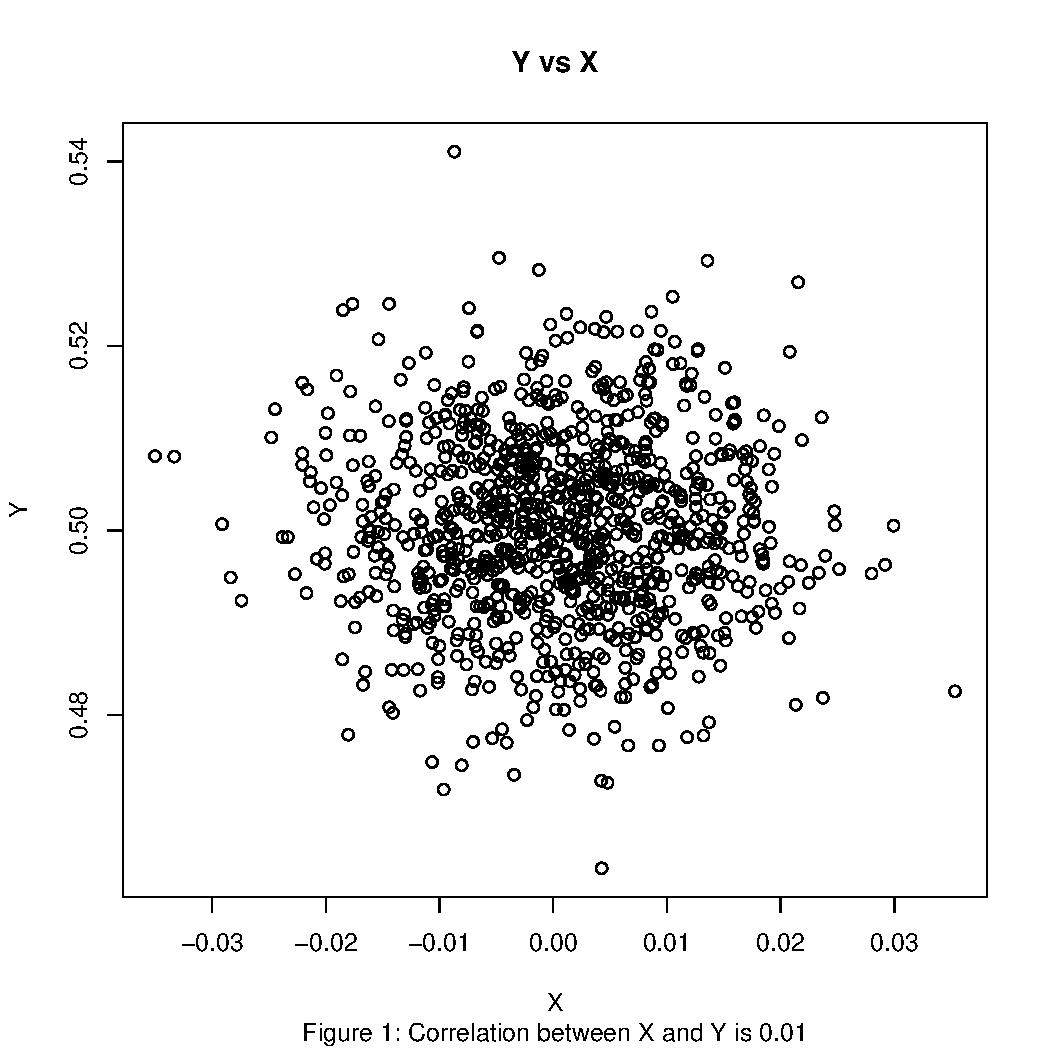
\includegraphics[width=4in]{figure/p1Plot-1} 
\begin{kframe}\begin{alltt}
\hlkwd{plot}\hlstd{(N.p1, ps,}
     \hlkwc{main} \hlstd{=} \hlstr{"P-value vs Number of Observations"}\hlstd{,}
     \hlkwc{sub} \hlstd{=} \hlstr{"Figure 2"}\hlstd{,}
     \hlkwc{ylab} \hlstd{=} \hlstr{"P-value"}\hlstd{,}
     \hlkwc{xlab} \hlstd{=} \hlstr{"Number of Observations"}
\hlstd{)}
\hlkwd{abline}\hlstd{(}\hlkwc{h} \hlstd{=} \hlnum{.05}\hlstd{)}
\end{alltt}
\end{kframe}
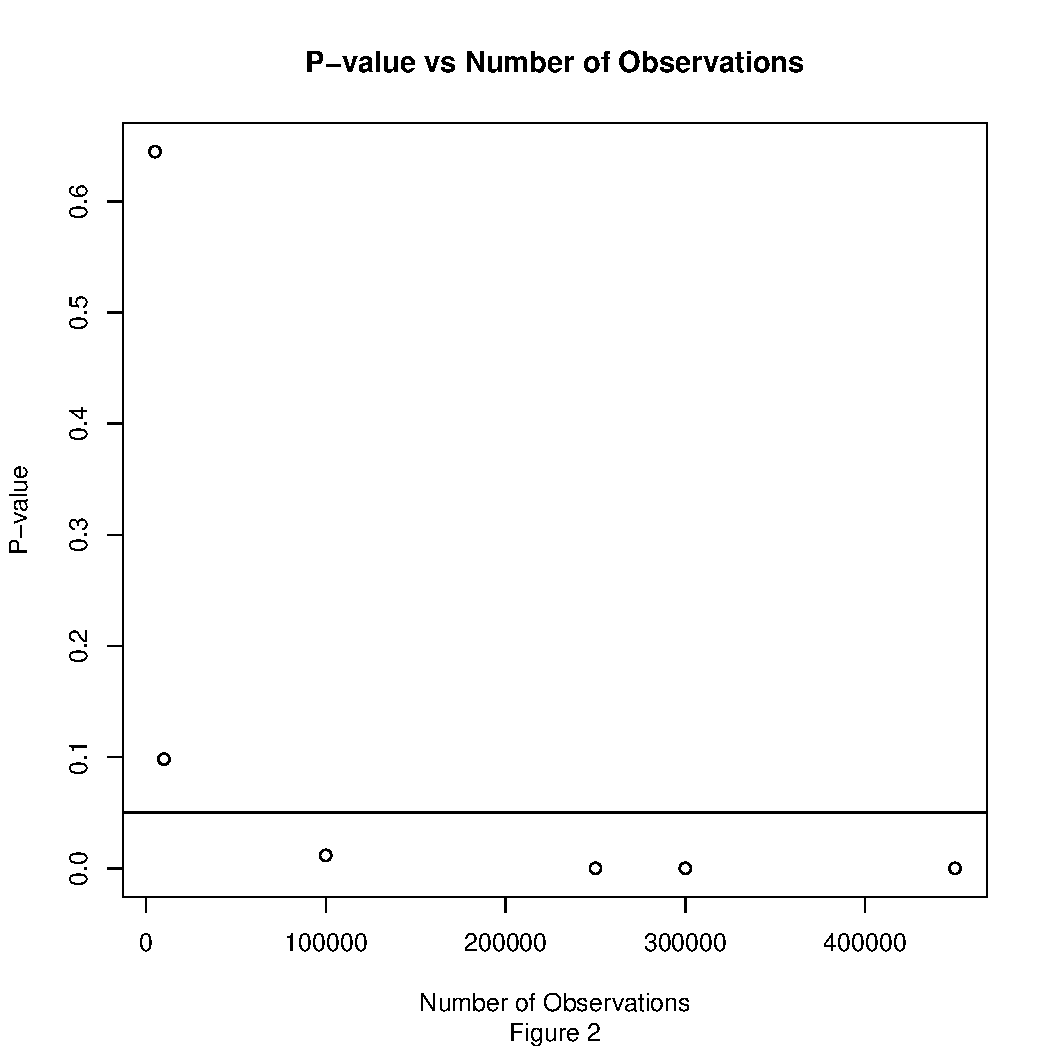
\includegraphics[width=4in]{figure/p1Plot-2} 

\end{knitrout}
\end{center}

\noindent We modeled X and $e$ such that both were normal with mean 0 and standard deviation 0.01. We set the parameters $a_{0}$ and $a_{1}$ to 0.5 and 0.01, respectively, such that $Y = 0.5 + 0.01*X + e$. The relationship between X and Y is weak, as seen in Figure 1. The plotted values form a cloud, indicating the weak correlation of 0.01 (we only plotted the first 1000 Xs and Ys due to the large number of data generated).  We generated datasets for samples of increasing size, from 5000 to 450000, and plotted the p-values of X for each of the $6$ trials in Figure 2. A horizontal line was drawn at a p-value of 0.05, the common threshold for rejecting the null hypothesis. The relationship is consistently statistically significant after 100000 samples, which shows that as the sample size increases, even weak relationships will be shown to be significant. Therefore, low p-values do not necessarily imply an important assocation between two variables. \\

\section*{Problem 2}
\subsection*{Part a}
\begin{knitrout}
\definecolor{shadecolor}{rgb}{0.969, 0.969, 0.969}\color{fgcolor}\begin{kframe}
\begin{alltt}
\hlkwd{set.seed}\hlstd{(}\hlnum{08544}\hlstd{)}
\hlstd{N.p2} \hlkwb{<-} \hlnum{1000}

\hlstd{x1} \hlkwb{<-} \hlkwd{rbinom}\hlstd{(N.p2,} \hlkwc{size} \hlstd{=} \hlnum{1}\hlstd{,} \hlkwc{prob} \hlstd{=} \hlnum{.056}\hlstd{)}
\hlstd{x2} \hlkwb{<-} \hlkwd{rnorm}\hlstd{(N.p2, (}\hlnum{5} \hlopt{-} \hlstd{x1}\hlopt{*}\hlnum{3}\hlstd{),} \hlnum{1.5}\hlstd{)}
\hlstd{y} \hlkwb{<-} \hlkwd{plogis}\hlstd{(x2} \hlopt{-} \hlnum{6}\hlstd{)}
\end{alltt}
\end{kframe}
\end{knitrout}
\noindent We completed Problem 2b prior to 2a, which is why the code is nearly identical. The creation of the dataset is described in 2b. The correlation between $X_{1}$ and $Y$ is -0.252, while the coefficient on $X_{1}$ from the regression is 0.191, as required.\\ 

\subsection*{Part b}
\begin{knitrout}
\definecolor{shadecolor}{rgb}{0.969, 0.969, 0.969}\color{fgcolor}\begin{kframe}
\begin{alltt}
\hlkwd{set.seed}\hlstd{(}\hlnum{08544}\hlstd{)}

\hlstd{asian} \hlkwb{<-} \hlkwd{rbinom}\hlstd{(N.p2,} \hlkwc{size} \hlstd{=} \hlnum{1}\hlstd{,} \hlkwc{prob} \hlstd{=} \hlnum{.056}\hlstd{)}
\hlstd{personality} \hlkwb{<-} \hlkwd{rnorm}\hlstd{(N.p2, (}\hlnum{5} \hlopt{-} \hlstd{asian}\hlopt{*}\hlnum{3}\hlstd{),} \hlnum{1.5}\hlstd{)}
\hlstd{harvard} \hlkwb{<-} \hlkwd{plogis}\hlstd{(personality} \hlopt{-} \hlnum{6}\hlstd{)}
\end{alltt}
\end{kframe}
\end{knitrout}

\noindent We chose to comment on the Harvard Circut Court decision on admission of Asian American applicants. Here, $X_{1}$ is Bernoulli variable that flags a candidate as Asian or not (5.6\% of the U.S. population is Asian). $X_{2}$ is the `personality score' as described in the brief. $X_{2}$ is normally distributed with mean 5 and standard deviation 1.5 if a candidate is non-Asian. If the candidate is Asian, the `personality score' is lower, with $X_{2}$ normally distributed with mean 2 and standard deviation 1.5. Y is the probability of acceptance to Harvard based on the personality score (which is lower for Asian applicants). We can see that the `personality score' is a lurking variable. The correlation between Asian and Harvard is -0.252. However, for a constant `personality score,' the coefficient on Asian is 0.191. \\

\section*{Problem 3}
\subsection*{Part a}
\begin{figure}[h!]
\centering
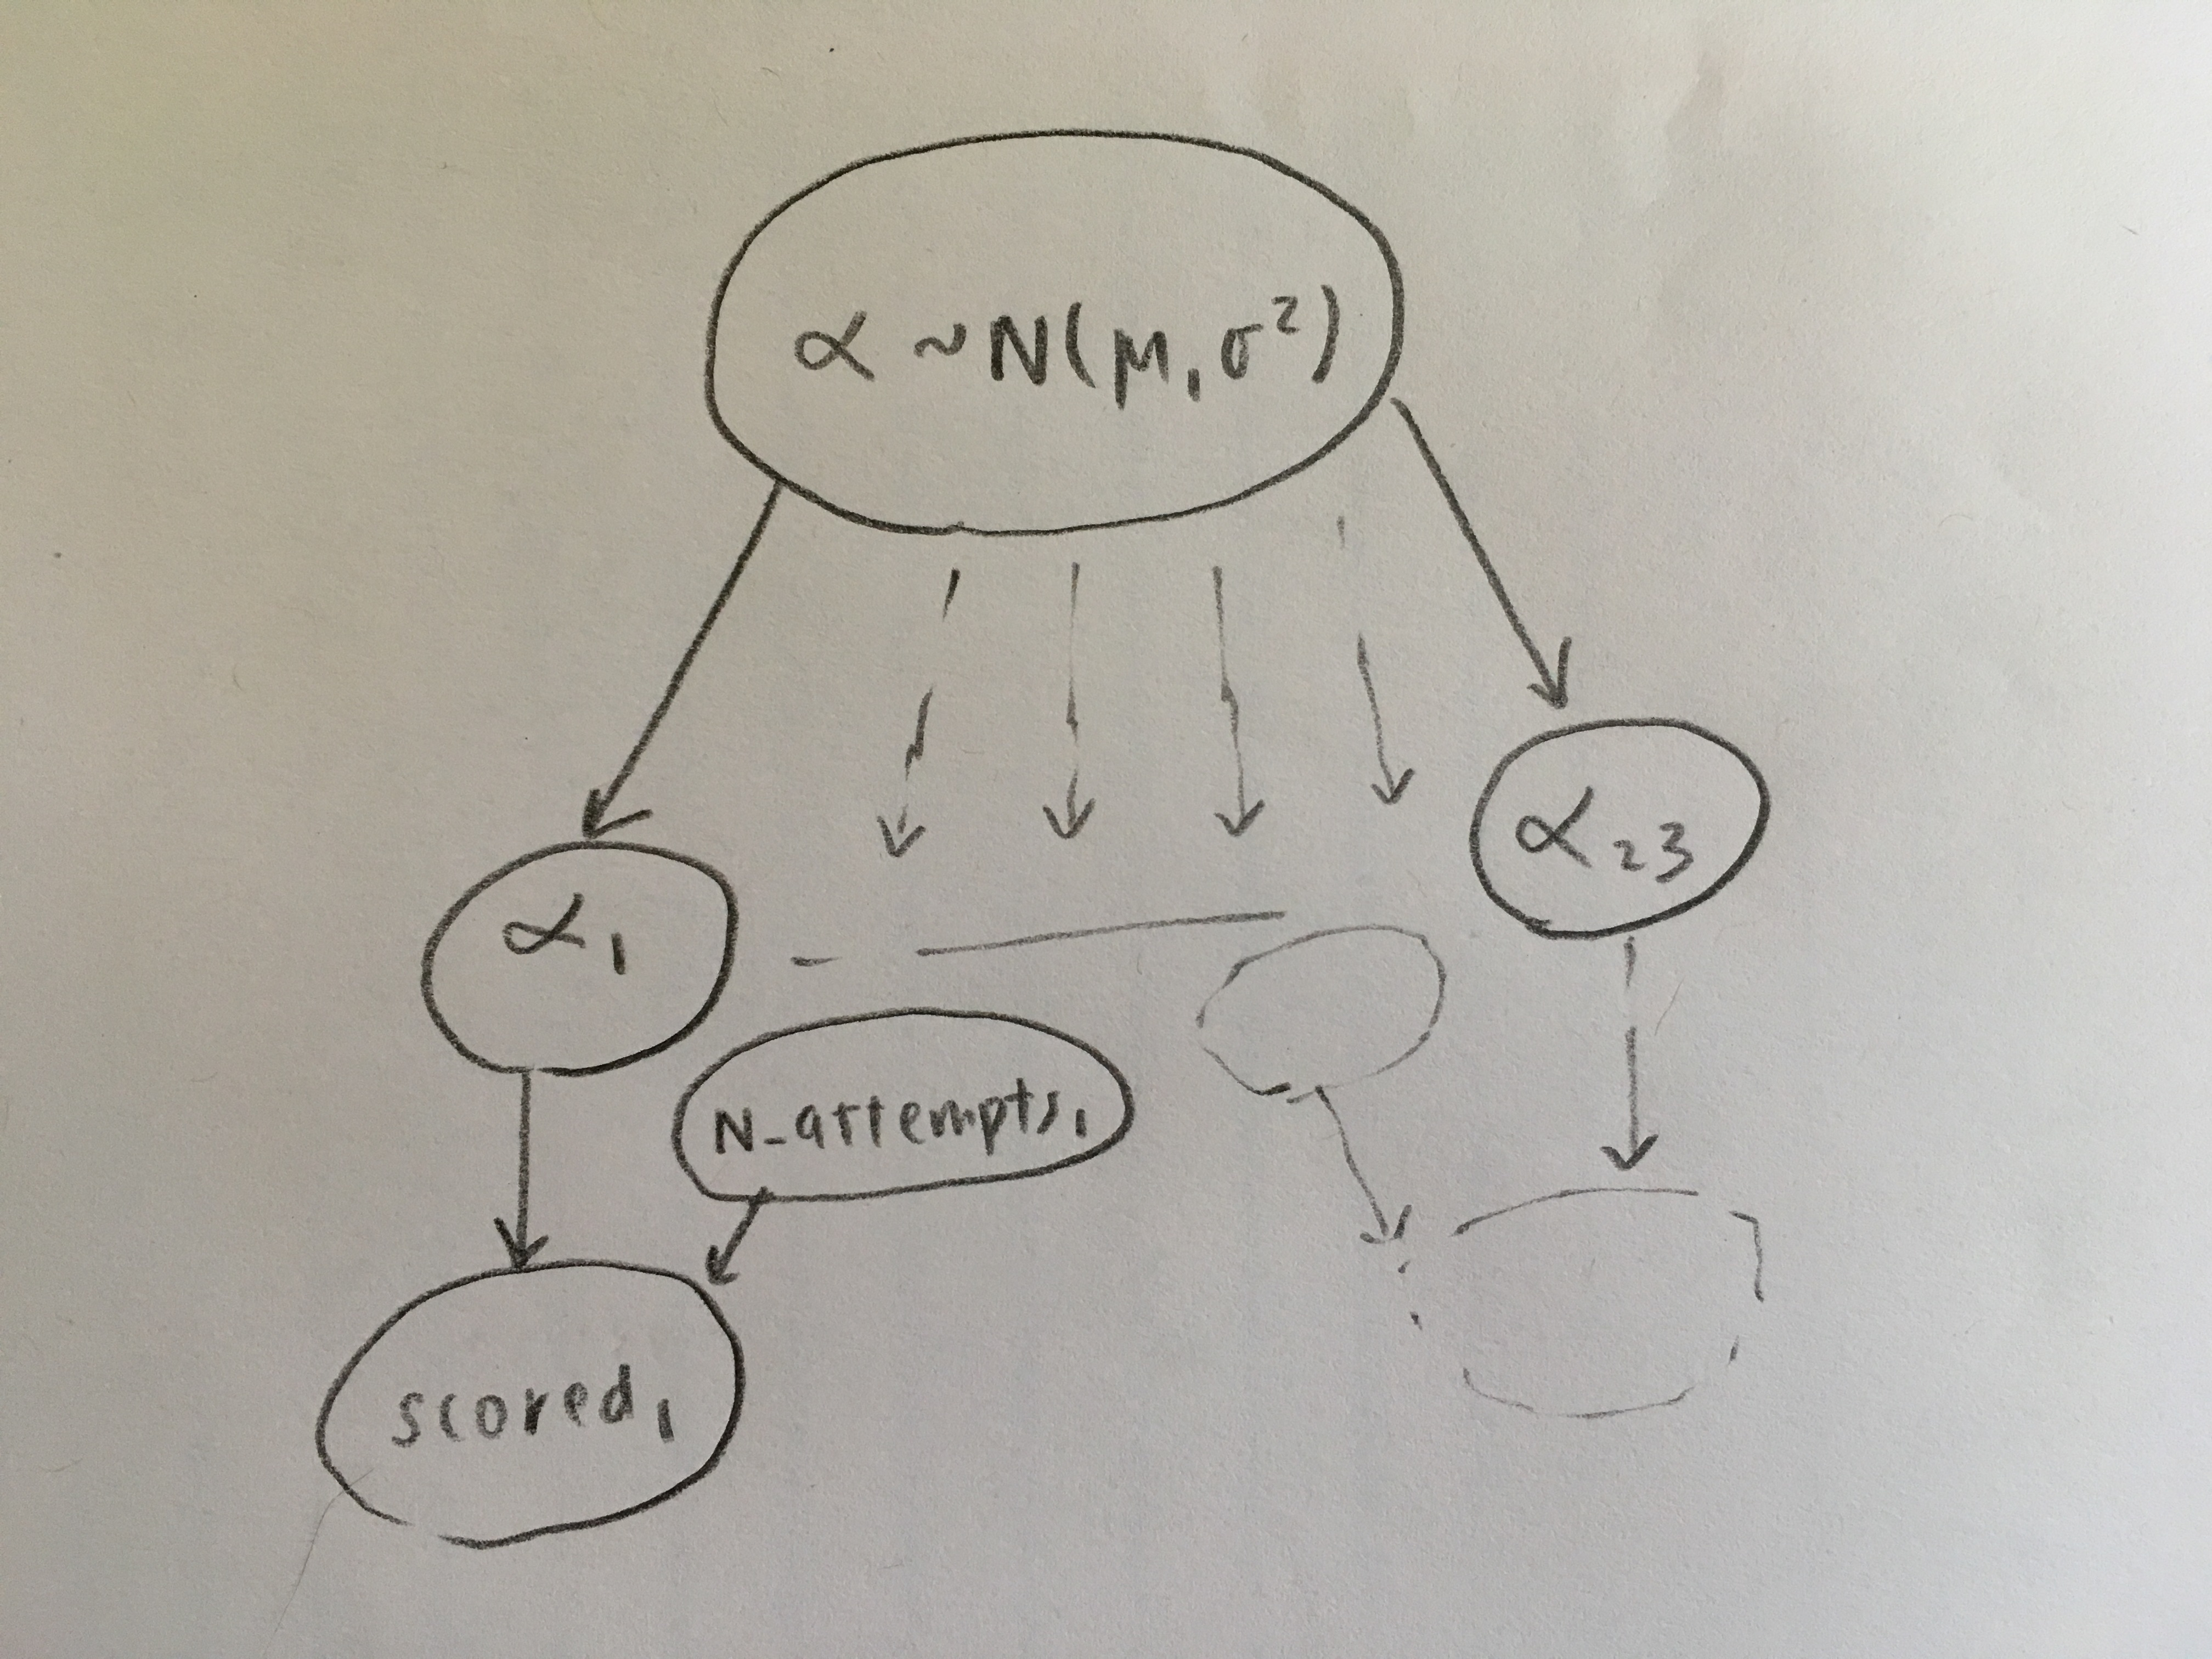
\includegraphics[scale=.08]{/Users/mikakoinaba/Desktop/sml310_mp1/p3a.jpg}
\end{figure}
\noindent Shown in the diagram above, the partial-pooling hierarchical model would make sense if Shaq had a different probablity of scoring on different days. We assumed skill level is normally distributed ($\alpha$), and each game Shaq has a different skill level from this distribution ($\alpha_i$). Each $\alpha_i$ influences the probability of scoring for that game in addition to the number of attempts. \\ \pagebreak

\subsection*{Part b}
\begin{knitrout}
\definecolor{shadecolor}{rgb}{0.969, 0.969, 0.969}\color{fgcolor}\begin{kframe}
\begin{alltt}
\hlstd{lines} \hlkwb{<-}
\hlstr{"Game   Scored  N.Attempts
1   4   5
2   5   11
3   5   14
4   5   12
5   2   7
6   7   10
7   6   14
8   9   15
9   4   12
10  1   4
11  13  27
12  5   17
13  6   12
14  9   9
15  7   12
16  3   10
17  8   12
18  1   6
19  18  39
20  3   13
21  10  17
22  1   6
23  3   12"}
\hlstd{con} \hlkwb{<-} \hlkwd{textConnection}\hlstd{(lines)}
\hlstd{shaq} \hlkwb{<-} \hlkwd{read.csv}\hlstd{(con,} \hlkwc{sep}\hlstd{=}\hlstr{""}\hlstd{)}
\hlstd{shaq}

\hlstd{shaq_model_stanPartial} \hlkwb{<-} \hlstr{"
data\{
  // data supplied
  int<lower=0> N; // game number, must be positive
  int scored[N]; // array of scores indexed by game
  int attempted[N]; // array of number of attempts indexed by game
\}

parameters\{
  real mu; // overall average skill level
  real<lower=0> sigma; // overall stdev of skill level, lower bounded by 0
  vector[N] alpha_norm; // array of `zscores' / number of stdev away from mean
                        // indexed by game
\}

transformed parameters\{
  real alpha[N]; // array of average skill level, produced using alpha_norm
                 // indexed by game

  // loop populates alpha from ~N(mu, sigma^2)
  for(n in 1:N)
    alpha[n] = mu + sigma * alpha_norm[n];
\}

model\{
  alpha_norm ~ normal(0, 1);
  scored ~ binomial(attempted, inv_logit(alpha));
  // scored is the sum of n Bernoulli RVs, each with a probability determined by alpha
  // n determined by the number of attempted shots
\}"}

\hlstd{adaptSteps} \hlkwb{=} \hlnum{1000}            \hlcom{# Number of steps to "tune" the samplers.}
\hlstd{burnInSteps} \hlkwb{=} \hlnum{5000}           \hlcom{# Number of steps to "burn-in" the samplers.}
\hlstd{nChains} \hlkwb{=} \hlnum{3}                  \hlcom{# Number of chains to run.}
\hlstd{numSavedSteps}\hlkwb{=}\hlnum{12000}          \hlcom{# Total number of steps in chains to save.}
\hlstd{thinSteps}\hlkwb{=}\hlnum{10}                 \hlcom{# Number of steps to "thin" (1=keep every step).}

\hlstd{shaq_model_stanPartial} \hlkwb{<-} \hlkwd{stan_model}\hlstd{(}\hlkwc{model_code} \hlstd{= shaq_model_stanPartial,}
                                     \hlkwc{model_name} \hlstd{=} \hlstr{"shaq_model_stanPartial"}\hlstd{)}
\hlstd{shaqPartial_fit} \hlkwb{<-} \hlkwd{sampling}\hlstd{(}\hlkwc{object}\hlstd{=shaq_model_stanPartial,}
                      \hlkwc{data} \hlstd{=} \hlkwd{list}\hlstd{(}\hlkwc{N}\hlstd{=}\hlkwd{nrow}\hlstd{(shaq),} \hlkwc{scored}\hlstd{=shaq}\hlopt{$}\hlstd{Scored,}
                                  \hlkwc{attempted} \hlstd{= shaq}\hlopt{$}\hlstd{N.Attempts),}
                      \hlkwc{chains} \hlstd{= nChains,}
                      \hlkwc{iter} \hlstd{= (}\hlkwd{ceiling}\hlstd{(numSavedSteps}\hlopt{/}\hlstd{nChains)}\hlopt{*}\hlstd{thinSteps}
                               \hlopt{+} \hlstd{burnInSteps),}
                      \hlkwc{warmup} \hlstd{= burnInSteps,}
                      \hlkwc{thin} \hlstd{= thinSteps,}
                      \hlkwc{init} \hlstd{=} \hlstr{"random"}\hlstd{)}

\hlstd{samplesPartial} \hlkwb{<-} \hlkwd{extract}\hlstd{(shaqPartial_fit)}
\hlstd{good} \hlkwb{<-} \hlkwd{plogis}\hlstd{(}\hlkwd{mean}\hlstd{(samplesPartial}\hlopt{$}\hlstd{mu)} \hlopt{+} \hlnum{2} \hlopt{*} \hlkwd{mean}\hlstd{(samplesPartial}\hlopt{$}\hlstd{sigma))}
\hlstd{bad} \hlkwb{<-} \hlkwd{plogis}\hlstd{(}\hlkwd{mean}\hlstd{(samplesPartial}\hlopt{$}\hlstd{mu)} \hlopt{-} \hlnum{2} \hlopt{*} \hlkwd{mean}\hlstd{(samplesPartial}\hlopt{$}\hlstd{sigma))}
\end{alltt}
\end{kframe}
\end{knitrout}
\begin{center}
\begin{knitrout}
\definecolor{shadecolor}{rgb}{0.969, 0.969, 0.969}\color{fgcolor}\begin{kframe}
\begin{alltt}
\hlkwd{hist}\hlstd{(samplesPartial}\hlopt{$}\hlstd{mu,} \hlkwc{main} \hlstd{=} \hlstr{"Mu"}\hlstd{,} \hlkwc{xlab} \hlstd{=} \hlstr{"Skill Level"}\hlstd{)}
\end{alltt}
\end{kframe}
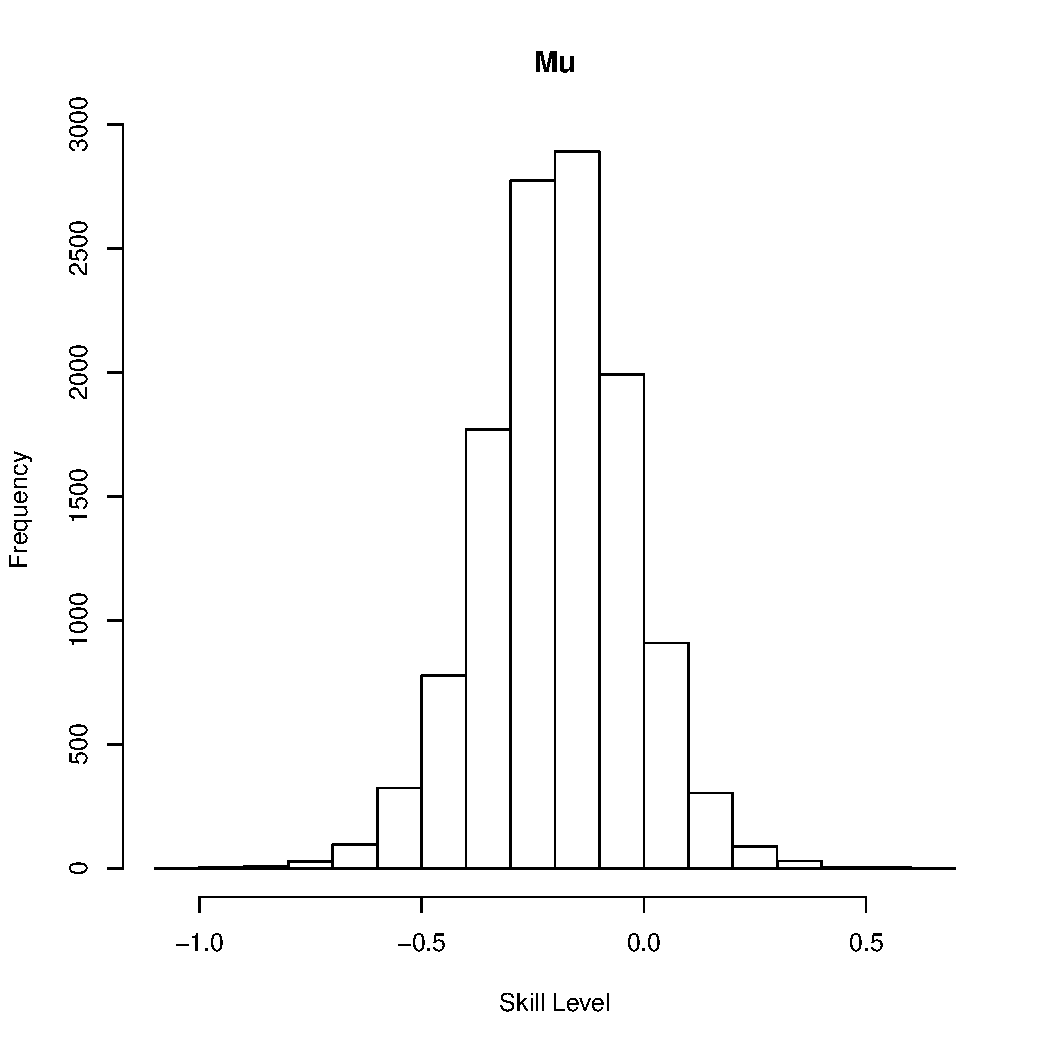
\includegraphics[width=4in]{figure/p3bHist-1} 
\begin{kframe}\begin{alltt}
\hlkwd{hist}\hlstd{(samplesPartial}\hlopt{$}\hlstd{sigma,} \hlkwc{main} \hlstd{=} \hlstr{"Sigma"}\hlstd{,} \hlkwc{xlab} \hlstd{=} \hlstr{"Skill Level"}\hlstd{)}
\end{alltt}
\end{kframe}
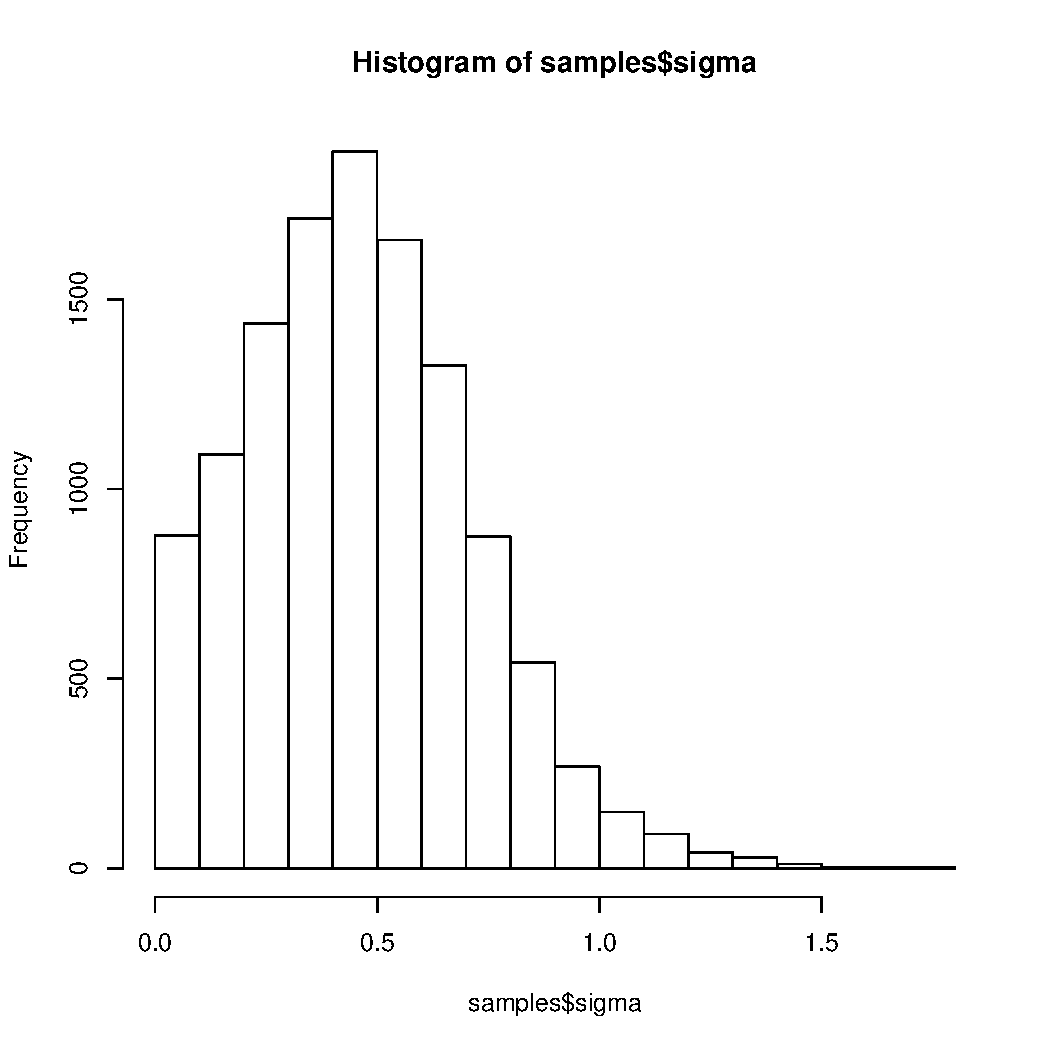
\includegraphics[width=4in]{figure/p3bHist-2} 

\end{knitrout}
\end{center}
\noindent The posterior distribution for mu and sigma were displayed. Given that 95\% of the data lies within 2 standard deviations from the mean, we found the probability of scoring on a particularly bad day (2 standard deviations lower than the mean) and on an especially good day (2 standard deviations above the mean). On a bad day, Shaq's probability of making a free throw is 0.245, and on a good day, Shaq's probability of making a free throw is 0.676. This is a difference of 0.43, which means that on a good day, Shaq has a 43.04 percentage point increase in scoring probability. This difference could alter the course of a basketball game, so we decided this was large enough to conclude that Shaq has good and bad days. Each line of Stan code was commented above. \\

\subsection*{Part c}
\begin{knitrout}
\definecolor{shadecolor}{rgb}{0.969, 0.969, 0.969}\color{fgcolor}\begin{kframe}
\begin{alltt}
\hlstd{shaq_model_stanNo} \hlkwb{<-} \hlstr{"
data\{
  int<lower=0> N; 
  int scored[N];
  int attempted[N];
\}

parameters\{
  real mu;
  vector[N] alpha_norm;
\}

transformed parameters\{
  real alpha[N];
  for(n in 1:N)
    alpha[n] = mu + 20 * alpha_norm[n];
\}

model\{
  alpha_norm ~ normal(0, 1);
  scored ~ binomial(attempted, inv_logit(alpha));
\}"}

\hlstd{adaptSteps} \hlkwb{=} \hlnum{1000}            \hlcom{# Number of steps to "tune" the samplers.}
\hlstd{burnInSteps} \hlkwb{=} \hlnum{5000}           \hlcom{# Number of steps to "burn-in" the samplers.}
\hlstd{nChains} \hlkwb{=} \hlnum{3}                  \hlcom{# Number of chains to run.}
\hlstd{numSavedSteps}\hlkwb{=}\hlnum{12000}          \hlcom{# Total number of steps in chains to save.}
\hlstd{thinSteps}\hlkwb{=}\hlnum{10}                 \hlcom{# Number of steps to "thin" (1=keep every step).}

\hlstd{shaq_model_stanNo} \hlkwb{<-} \hlkwd{stan_model}\hlstd{(}\hlkwc{model_code} \hlstd{= shaq_model_stanNo,}
                                \hlkwc{model_name} \hlstd{=} \hlstr{"shaq_model_stanNo"}\hlstd{)}
\hlstd{shaqNo_fit} \hlkwb{<-} \hlkwd{sampling}\hlstd{(}\hlkwc{object}\hlstd{=shaq_model_stanNo,}
                      \hlkwc{data} \hlstd{=} \hlkwd{list}\hlstd{(}\hlkwc{N}\hlstd{=}\hlkwd{nrow}\hlstd{(shaq),} \hlkwc{scored}\hlstd{=shaq}\hlopt{$}\hlstd{Scored,}
                                  \hlkwc{attempted} \hlstd{= shaq}\hlopt{$}\hlstd{N.Attempts),}
                      \hlkwc{chains} \hlstd{= nChains ,}
                      \hlkwc{iter} \hlstd{= (} \hlkwd{ceiling}\hlstd{(numSavedSteps}\hlopt{/}\hlstd{nChains)}\hlopt{*}\hlstd{thinSteps}
                               \hlopt{+}\hlstd{burnInSteps ) ,}
                      \hlkwc{warmup} \hlstd{= burnInSteps ,}
                      \hlkwc{thin} \hlstd{= thinSteps ,}
                      \hlkwc{init} \hlstd{=} \hlstr{"random"} \hlstd{)}

\hlstd{samplesNo} \hlkwb{<-} \hlkwd{extract}\hlstd{(shaqNo_fit)}
\end{alltt}
\end{kframe}
\end{knitrout}
\begin{center}
\begin{knitrout}
\definecolor{shadecolor}{rgb}{0.969, 0.969, 0.969}\color{fgcolor}\begin{kframe}
\begin{alltt}
\hlstd{N.p3} \hlkwb{<-} \hlnum{23}
\hlstd{conf_dataNo} \hlkwb{<-} \hlkwd{data.frame}\hlstd{(}\hlkwc{games} \hlstd{=} \hlnum{1}\hlopt{:}\hlstd{N.p3,} \hlkwc{mean} \hlstd{=} \hlnum{NA}\hlstd{,} \hlkwc{upper} \hlstd{=} \hlnum{NA}\hlstd{,} \hlkwc{lower} \hlstd{=} \hlnum{NA}\hlstd{)}

\hlkwa{for} \hlstd{(i} \hlkwa{in} \hlnum{1}\hlopt{:}\hlstd{N.p3)\{}
  \hlstd{conf_dataNo[i,} \hlstr{"mean"}\hlstd{]} \hlkwb{=} \hlkwd{mean}\hlstd{(samplesNo}\hlopt{$}\hlstd{alpha[, i])}
  \hlstd{conf_dataNo[i,} \hlstr{"upper"}\hlstd{]} \hlkwb{=} \hlkwd{mean}\hlstd{(samplesNo}\hlopt{$}\hlstd{alpha[, i])} \hlopt{+} \hlnum{2} \hlopt{*} \hlkwd{sd}\hlstd{(samplesNo}\hlopt{$}\hlstd{alpha[, i])}
  \hlstd{conf_dataNo[i,} \hlstr{"lower"}\hlstd{]} \hlkwb{=} \hlkwd{mean}\hlstd{(samplesNo}\hlopt{$}\hlstd{alpha[, i])} \hlopt{-} \hlnum{2} \hlopt{*} \hlkwd{sd}\hlstd{(samplesNo}\hlopt{$}\hlstd{alpha[, i])}
\hlstd{\}}

\hlkwd{ggplot}\hlstd{(conf_dataNo,} \hlkwd{aes}\hlstd{(}\hlkwc{y} \hlstd{= mean,} \hlkwc{x} \hlstd{= games))} \hlopt{+}
  \hlkwd{geom_errorbar}\hlstd{(}\hlkwd{aes}\hlstd{(}\hlkwc{ymin}\hlstd{=lower,} \hlkwc{ymax}\hlstd{=upper))} \hlopt{+} \hlkwd{ggtitle}\hlstd{(}\hlstr{"95% Intervals: No-Pooling"}\hlstd{)} \hlopt{+}
  \hlkwd{theme}\hlstd{(}\hlkwc{plot.title} \hlstd{=} \hlkwd{element_text}\hlstd{(}\hlkwc{hjust} \hlstd{=} \hlnum{0.5}\hlstd{))} \hlopt{+}
  \hlkwd{ylab}\hlstd{(}\hlstr{"Skill Level"}\hlstd{)} \hlopt{+} \hlkwd{xlab}\hlstd{(}\hlstr{"Game Number"}\hlstd{)}
\end{alltt}
\end{kframe}
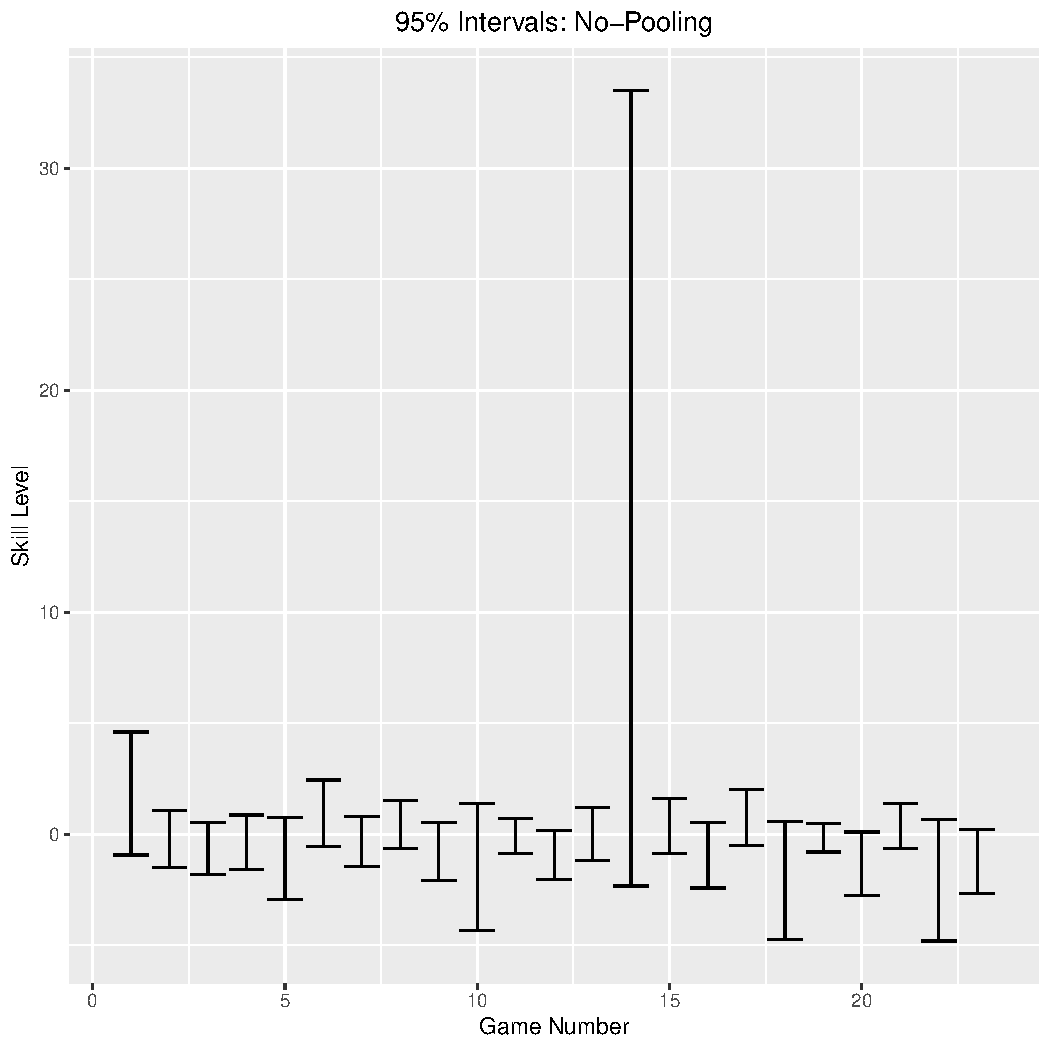
\includegraphics[width=4in]{figure/p3cNoData-1} 

\end{knitrout}

\begin{knitrout}
\definecolor{shadecolor}{rgb}{0.969, 0.969, 0.969}\color{fgcolor}\begin{kframe}
\begin{alltt}
\hlstd{conf_dataPartial} \hlkwb{<-} \hlkwd{data.frame}\hlstd{(}\hlkwc{games} \hlstd{=} \hlnum{1}\hlopt{:}\hlstd{N.p3,} \hlkwc{mean} \hlstd{=} \hlnum{NA}\hlstd{,} \hlkwc{upper} \hlstd{=} \hlnum{NA}\hlstd{,} \hlkwc{lower} \hlstd{=} \hlnum{NA}\hlstd{)}

\hlkwa{for} \hlstd{(i} \hlkwa{in} \hlnum{1}\hlopt{:}\hlstd{N.p3)\{}
  \hlstd{conf_dataPartial[i,} \hlstr{"mean"}\hlstd{]} \hlkwb{=} \hlkwd{mean}\hlstd{(samplesPartial}\hlopt{$}\hlstd{alpha[, i])}
  \hlstd{conf_dataPartial[i,} \hlstr{"upper"}\hlstd{]} \hlkwb{=} \hlkwd{mean}\hlstd{(samplesPartial}\hlopt{$}\hlstd{alpha[, i])} \hlopt{+}
                                 \hlnum{2} \hlopt{*} \hlkwd{sd}\hlstd{(samplesPartial}\hlopt{$}\hlstd{alpha[, i])}
  \hlstd{conf_dataPartial[i,} \hlstr{"lower"}\hlstd{]} \hlkwb{=} \hlkwd{mean}\hlstd{(samplesPartial}\hlopt{$}\hlstd{alpha[, i])} \hlopt{-}
                                 \hlnum{2} \hlopt{*} \hlkwd{sd}\hlstd{(samplesPartial}\hlopt{$}\hlstd{alpha[, i])}
\hlstd{\}}

\hlkwd{ggplot}\hlstd{(conf_dataPartial,} \hlkwd{aes}\hlstd{(}\hlkwc{x} \hlstd{= games,} \hlkwc{y} \hlstd{= mean))} \hlopt{+}
  \hlkwd{geom_errorbar}\hlstd{(}\hlkwd{aes}\hlstd{(}\hlkwc{ymin}\hlstd{=lower,} \hlkwc{ymax}\hlstd{=upper))} \hlopt{+}
  \hlkwd{ggtitle}\hlstd{(}\hlstr{"95% Intervals: Partial-Pooling"}\hlstd{)} \hlopt{+}
  \hlkwd{theme}\hlstd{(}\hlkwc{plot.title} \hlstd{=} \hlkwd{element_text}\hlstd{(}\hlkwc{hjust} \hlstd{=} \hlnum{0.5}\hlstd{))} \hlopt{+}
  \hlkwd{ylab}\hlstd{(}\hlstr{"Skill Level"}\hlstd{)} \hlopt{+} \hlkwd{xlab}\hlstd{(}\hlstr{"Game Number"}\hlstd{)}
\end{alltt}
\end{kframe}
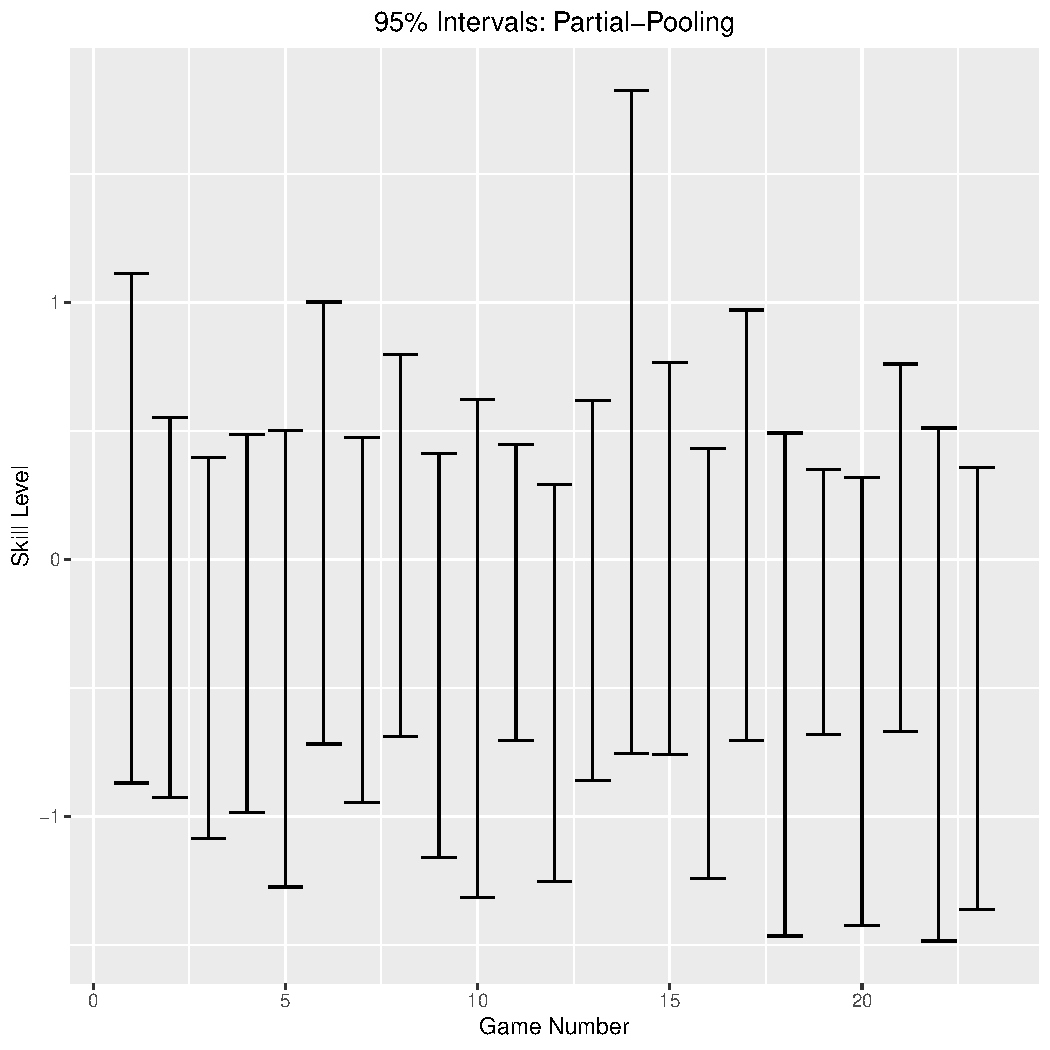
\includegraphics[width=4in]{figure/p3cPartial-1} 

\end{knitrout}
\end{center}

\begin{knitrout}
\definecolor{shadecolor}{rgb}{0.969, 0.969, 0.969}\color{fgcolor}\begin{kframe}
\begin{alltt}
\hlstd{shaq_model_stanComplete} \hlkwb{<-} \hlstr{"
data\{
  int<lower=0> N;
  int scored[N];
  int attempted[N];
\}

parameters\{
  real mu;
  vector[N] alpha_norm;
\}

transformed parameters\{
  real alpha[N];
  for(n in 1:N)
    alpha[n] = mu + 0 * alpha_norm[n];
\}

model\{
  alpha_norm ~ normal(0, 1);
  scored ~ binomial(attempted, inv_logit(alpha));
\}"}

\hlstd{shaq_model_stanComplete} \hlkwb{<-} \hlkwd{stan_model}\hlstd{(}\hlkwc{model_code} \hlstd{= shaq_model_stanComplete,}
                                      \hlkwc{model_name} \hlstd{=} \hlstr{"shaq_model_stanComplete"}\hlstd{)}
\hlstd{shaqComplete_fit} \hlkwb{<-} \hlkwd{sampling}\hlstd{(}\hlkwc{object}\hlstd{=shaq_model_stanComplete,}
                      \hlkwc{data} \hlstd{=} \hlkwd{list}\hlstd{(}\hlkwc{N}\hlstd{=}\hlkwd{nrow}\hlstd{(shaq),} \hlkwc{scored}\hlstd{=shaq}\hlopt{$}\hlstd{Scored,}
                                  \hlkwc{attempted} \hlstd{= shaq}\hlopt{$}\hlstd{N.Attempts),}
                      \hlkwc{chains} \hlstd{= nChains ,}
                      \hlkwc{iter} \hlstd{= (} \hlkwd{ceiling}\hlstd{(numSavedSteps}\hlopt{/}\hlstd{nChains)}\hlopt{*}\hlstd{thinSteps}
                               \hlopt{+}\hlstd{burnInSteps ) ,}
                      \hlkwc{warmup} \hlstd{= burnInSteps ,}
                      \hlkwc{thin} \hlstd{= thinSteps ,}
                      \hlkwc{init} \hlstd{=} \hlstr{"random"} \hlstd{)}

\hlstd{samplesComplete} \hlkwb{<-} \hlkwd{extract}\hlstd{(shaqComplete_fit)}
\end{alltt}
\end{kframe}
\end{knitrout}

\begin{center}
\begin{knitrout}
\definecolor{shadecolor}{rgb}{0.969, 0.969, 0.969}\color{fgcolor}\begin{kframe}
\begin{alltt}
\hlstd{conf_dataComplete} \hlkwb{<-} \hlkwd{data.frame}\hlstd{(}\hlkwc{games} \hlstd{=} \hlnum{1}\hlopt{:}\hlstd{N.p3,} \hlkwc{mean} \hlstd{=} \hlnum{NA}\hlstd{,} \hlkwc{upper} \hlstd{=} \hlnum{NA}\hlstd{,} \hlkwc{lower} \hlstd{=} \hlnum{NA}\hlstd{)}

\hlkwa{for} \hlstd{(i} \hlkwa{in} \hlnum{1}\hlopt{:}\hlstd{N.p3)\{}
  \hlstd{conf_dataComplete[i,} \hlstr{"mean"}\hlstd{]} \hlkwb{=} \hlkwd{mean}\hlstd{(samplesComplete}\hlopt{$}\hlstd{alpha[, i])}
  \hlstd{conf_dataComplete[i,} \hlstr{"upper"}\hlstd{]} \hlkwb{=} \hlkwd{mean}\hlstd{(samplesComplete}\hlopt{$}\hlstd{alpha[, i])} \hlopt{+}
                                  \hlnum{2} \hlopt{*} \hlkwd{sd}\hlstd{(samplesComplete}\hlopt{$}\hlstd{alpha[, i])}
  \hlstd{conf_dataComplete[i,} \hlstr{"lower"}\hlstd{]} \hlkwb{=} \hlkwd{mean}\hlstd{(samplesComplete}\hlopt{$}\hlstd{alpha[, i])} \hlopt{-}
                                  \hlnum{2} \hlopt{*} \hlkwd{sd}\hlstd{(samplesComplete}\hlopt{$}\hlstd{alpha[, i])}
\hlstd{\}}

\hlkwd{ggplot}\hlstd{(conf_dataComplete,} \hlkwd{aes}\hlstd{(}\hlkwc{x} \hlstd{= games,} \hlkwc{y} \hlstd{= mean))} \hlopt{+}
  \hlkwd{geom_errorbar}\hlstd{(}\hlkwd{aes}\hlstd{(}\hlkwc{ymin}\hlstd{=lower,} \hlkwc{ymax}\hlstd{=upper))} \hlopt{+}
  \hlkwd{ggtitle}\hlstd{(}\hlstr{"95% Intervals: Complete-Pooling"}\hlstd{)} \hlopt{+}
  \hlkwd{theme}\hlstd{(}\hlkwc{plot.title} \hlstd{=} \hlkwd{element_text}\hlstd{(}\hlkwc{hjust} \hlstd{=} \hlnum{0.5}\hlstd{))} \hlopt{+}
  \hlkwd{ylab}\hlstd{(}\hlstr{"Skill Level"}\hlstd{)} \hlopt{+} \hlkwd{xlab}\hlstd{(}\hlstr{"Game Number"}\hlstd{)}
\end{alltt}
\end{kframe}
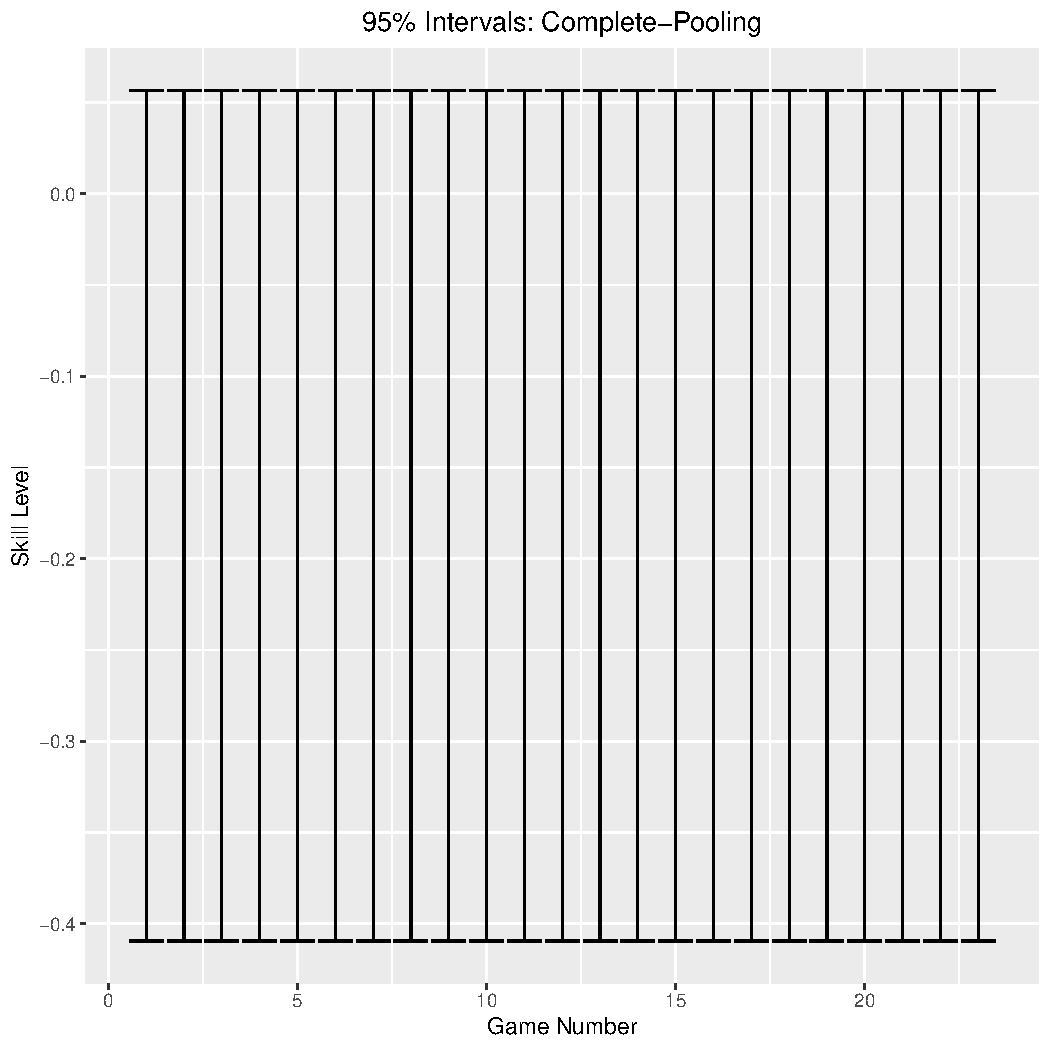
\includegraphics[width=4in]{figure/p3cCompleteData-1} 

\end{knitrout}
\end{center}

\noindent The 95\% predictive interval for each day was plotted for each of the three models, no-pooling, partial-pooling, and complete-pooling. The x-axis is the game number and the y-axis is the skill level. No-pooling assumes there is no connection between Shaq's skill level at each game. This translates to a very large sigma (in this case, 20). Partial-pooling assumes that Shaq's skill level differs at each game, dictated by the overall sigma (more specifically explained in 3a). Complete-pooling pools all the games into one, assuming that each game has the same skill level. This translates to a sigma of 0. \\

\noindent *Side note with respect to reproducibility - the image is in a folder on my Desktop, but with that commented out, everything else should be reproducibile. \\

\end{document}

